\lab{The Finite Element Method in Two Dimensions}{The Finite Element Method in Two Dimensions}
\label{lab:finite_element_2d}

In Lab \ref{lab:finite_element} we discussed some of the basic details of how the Finite Element Method works.
We demonstrated how a grid can be refined around areas of interest to give a more accurate approximation to a desired solution.
One of the other great strengths of the finite element method is that, when it is used in two or more dimensions, it is easily applied to unusually shaped domains.
There are a wide variety of elements that are commonly used, but the simplest elements are triangles.
Triangles are often used because they allow us to define continuous piecewise linear basis functions on their interiors without much trouble.

\section*{Working With Triangle Meshes}
There are a variety of ways to store triangle meshes.
We will present a simple one here.
To store a mesh we need to store several pieces of information.
We need to store the points used in the mesh.
We also need to store which points are connected to make the triangles that are part of the mesh we are studying.
Later, when working with boundary conditions, we will also need to know which nodes have fixed values (or some other sort of boundary condition, as the case may be).

It is common to store this information in arrays, one containing the $x$ and $y$ coordinates of each node in each of its rows and another containing the indices of the nodes that form the vertices of each triangle.

The following is a short example that divides the unit square up into triangles and returns arrays of the desired form.

\begin{lstlisting}
import numpy as np

def triangles(n):
    ''' Generate the indices of the triangles for a triangular mesh
    on a square grid of points.
    'n' is expected to be the number of nodes on each edge. '''
    # Make the indices for a single row.
    row = np.empty((2 * (n - 1), 3), dtype=np.int32)
    row[::2,0] = row[1::2,0] = row[::2,1] = np.arange(n-1)
    row[1::2,0] += 1
    row[::2,1] += n
    row[1::2,1] = row[::2,1]
    row[::2,2] = row[1::2,2] = row[1::2,0]
    row[1::2,2] += n
    # Now use broadcasting to make the indices for the square.
    return (row + np.arange(0, n * (n-1), n)[:,None,None]).reshape((-1,3))
\end{lstlisting}

Matplotlib's \li{triplot} function can be used to plot triangulations.
To plot the mesh generated by the above function, we can do the following:
\begin{lstlisting}
from matplotlib import pyplot as plt
n=5
x = np.linspace(0, 1, n)
x, y = map(np.ravel, np.meshgrid(x, x))
t = triangles(n)
plt.triplot(x, y, t, color='b')
plt.scatter(x, y, color='b')
plt.show()
\end{lstlisting}
This mesh is shown in figure \ref{fig:fem2d_square_triangulation}.

\begin{figure}
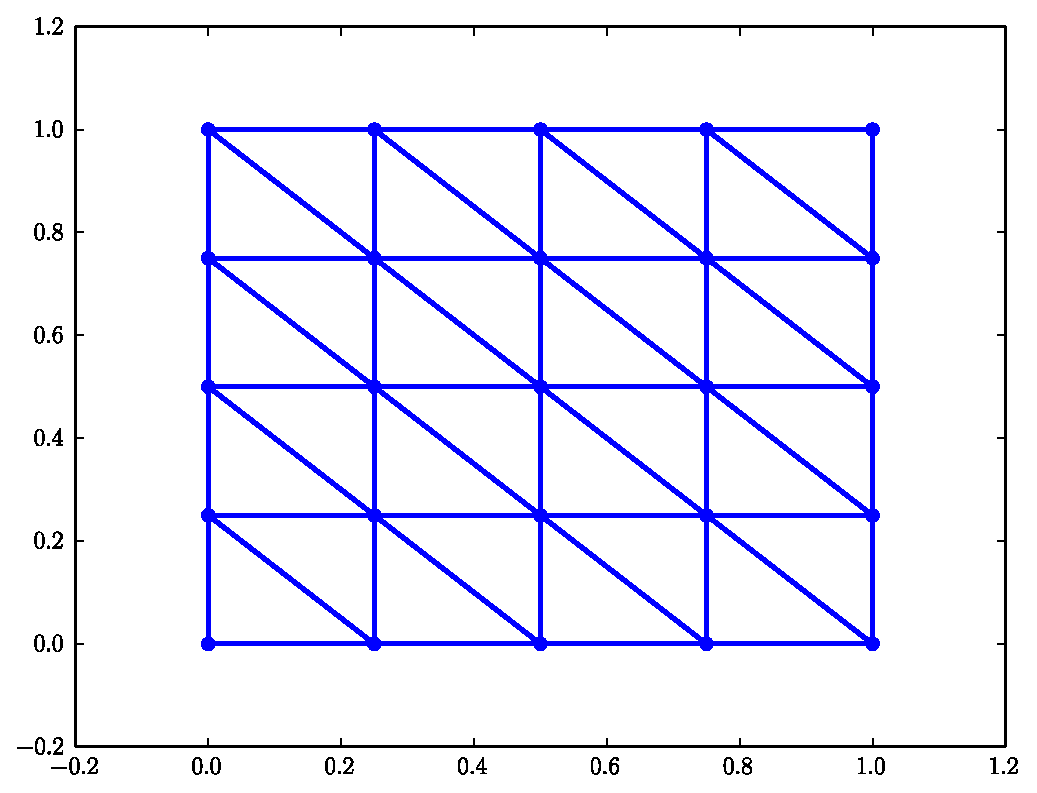
\includegraphics[width=\textwidth]{square_triangulation.pdf}
\caption{A triangulation of a square grid.}
\label{fig:fem2d_square_triangulation}
\end{figure}

Matplotlib and Mayavi both include the functionality to plot 3d surfaces based on a triangulation and the values of a function at the nodes of the triangulation.
For example, we can plot a piecewise linear function that is one at a single vertex and zero at every other vertex using Mayavi using the \li{triangular_mesh} function included in \li{mlab}.
\begin{lstlisting}
from mayavi import mlab as ml
n=5
x = np.linspace(0, 1, n)
x, y = np.meshgrid(x, x)
t = triangle_mesh(n)
vals = np.zeros(x.size)
vals[n**2 // 2] = 1
ml.triangular_mesh(x.ravel(), y.ravel(), vals, t)
ml.show()
\end{lstlisting}
The output from this code is shown in Figure \ref{fig:fem2d_basis_functions}.
These functions are often called "hat functions," and are often used as the basis functions for 2d finite element analysis on domains that can be represented as meshes of triangles.
These are the two dimensional analogues of the piecewise linear functions shown in Figure \ref{fig:FEM_one_basis_function}.
You may recall that, in the one-dimensional case, we could represent any function that was continuous and linear over each element as a sum of these basis functions.
The same is true in this case.
We can represent any continuous function that is linear on each triangle in the triangulation as a sum of these basis functions.
Strictly speaking, if $f$ is a continuous function that is linear on each of the triangles in the triangulation, $p_i$ are the vertices of the trianglulation, and $\phi_i$ are the basis functions corresponding to each vertex, we may say
\[f(x) = \sum_{i} f(p_i) \phi_i(x, y)\]

\begin{figure}
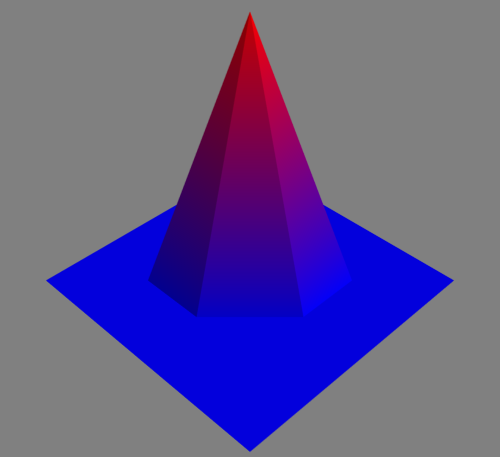
\includegraphics[width=\textwidth]{hat_function.png}
\caption{A hat function in two dimensions. Compare with the one dimensional hat function shown in Figure \ref{fig:FEM_one_basis_function}.}
\label{fig:fem2d_basis_functions}
\end{figure}

We can plot funcitons like this on triangulations using matplotlib as well.
The following code will plot the same basis function in matplotlib
\begin{lstlisting}
from mpl_toolkits.mplot3d import Axes3D
n=6
x = np.linspace(0, 1, n)
x, y = map(np.ravel, np.meshgrid(x, x))
t = triangles(n)
vals = np.random.rand(x.size)
fig = plt.figure()
ax = fig.add_subplot(1, 1, 1, projection='3d')
ax.plot_trisurf(x, y, vals, triangles=t)
plt.show()
\end{lstlisting}

\section*{Using Triangulations for Finite Element Analysis}

As was mentioned before, hat functions on triangulations are often used in Finite Element analysis.
When using the Finite element mehtod, regardless of the number of dimensions, it is necessary to transform a problem to its weak formulation.
This allows the approximation of the action of a PDE on a domain via the computation of integrals.
To begin, we will consider the differential operator
\[-\nabla \cdot \left(a\left(x\right) \nabla u\left(x\right)\right) + b\left(x\right) \cdot \nabla u\left(x\right) + c\left(x\right) u\left(x\right) = d\left(x\right)\]
on a triangulated domain $\Omega$.
For simplicity, we will first consider the case where $u$ is assumed to have Neumann boundary conditions.
The weak formulation of this problem on a function space $V$ is to find a function $u$ such that $a\left(u, v\right) = l\left(v\right)$ for all $v \in V$ with $a$ and $l$ defined as the following integral operators.
\begin{align*}
a\left(u, v\right) &= \int_\Omega \left( a\left(x\right) \nabla u\left(x\right) \cdot \nabla v\left(x\right) + \left(b\left(x\right) \cdot \nabla u\left(x\right)\right) v\left(x\right) + c\left(x\right) u\left(x\right) v\left(x\right) \right) dx\\
l\left(v\right) &= \int_\Omega d\left(x\right) v\left(x\right) dx
\end{align*}

We will find an approximate solution to the PDE that lies in the space $V$ of functions that are continuous and linear on each of the triangles in the triangulation of $\Omega$.
Let $\phi_i$ be the hat function centered at the $i$'th vertex of the triangulation of $\Omega$.
The $\phi_i$ are a basis for $V$, so we may say that we seek coefficients $u_i$ such that for any set of coefficients $v_i$,
\[a\left(\sum_i u_i \phi_i , \sum_j v_j \phi_j \right) = l\left(\sum_j v_j \phi_j\right)\]
Since $a$ is linear in its second term and $l$ is linear, this is equivalent to finding coefficients $u_i$ such that
\[a\left(\sum_i u_i \phi_i , \phi_j \right) = l\left(\phi_j\right)\]
Since $a$ is also linear in its first term, this is equivalent to finding $u_i$ such that
\[\sum_i u_i a\left(\phi_i, \phi_j\right) = l\left(\phi_j\right)\]
This problem can be represented as a linear system $A u = \Phi$ where $\Phi_j = l\left(\phi_j\right)$ and $A_{j, i} = a\left(\phi_i, \phi_j\right)$.
Generally speaking, this problem can be solved by construct the matrix $A$, and the vector $\Phi$, and then solving the resulting system.

\begin{info}
The matrix $A$ in the linear system constructed here is often referred to as the ``stiffness matrix."
The vector $\Phi$ is commonly known as the ``load vector."
\end{info}

\begin{info}
Notice that $a\left(\phi_i, \phi_j\right)$ depends entirely on the area where $\phi_i$ and $\phi_j$ are both nonzero.
If the supports of the functions $\phi_i$ and $\phi_j$ do not overlap, $a\left(\phi_i, \phi_j\right) = 0$.
Since only neighboring hat functions yield nonzero terms in the sum, the matrix $A$ is usually sparse.
\end{info}

\subsection*{Constructing the Stiffness Matrix and Load Vector}
It is not always easiest to construct the stiffness matrix and load vector by considering the basis functions one at a time.